\documentclass[titlepage]{article}
\usepackage{hyperref}
\usepackage{tikz}
\usepackage{enumerate}
\usepackage[T1]{fontenc}
\usepackage{listings}
\usepackage[superscript]{cite}
\usetikzlibrary{arrows,automata}

\lstset{
  language=C,
  aboveskip=3mm,
  belowskip=3mm,
  showstringspaces=false,
  columns=flexible,
  basicstyle={\small\ttfamily},
  numbers=none,
  keywordstyle=\color{blue},
  stringstyle=\color{green},
  breaklines=true,
  breakatwhitespace=true,
  tabsize=4,
  xleftmargin=.5in
}

\hypersetup{
  colorlinks,
  citecolor=black,
  linkcolor=black,
  urlcolor=black
}

\begin{document}
\title{TDT4205 Compiler Technology Problem Set 2}
\maketitle
\setcounter{secnumdepth}{0}

\section{Problem 1, Regular languages}
\begin{enumerate}[a)]
\item \leavevmode{\vspace{-\baselineskip}}\\
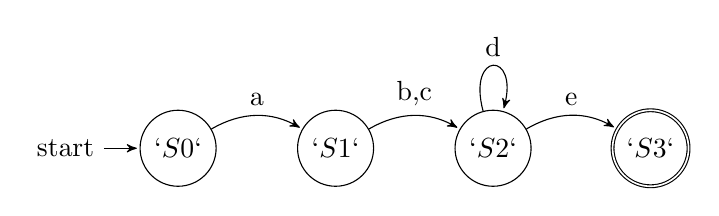
\begin{tikzpicture}[>=stealth',shorten >=1pt,auto,node distance=2cm]
  \node[initial,state]    (S)               {`$S0$`};
  \node[state]            (q1) [right of=S] {`$S1$`};
  \node[state]            (q2) [right of=q1]{`$S2$`};
  \node[state,accepting]  (q3) [right of=q2]{`$S3$`};

  \path[->] (S)  edge [bend left]  node {a}  (q1)
            (q1) edge [bend left]  node {b,c}(q2)
            (q2) edge [bend left]  node {e}  (q3)
                 edge [loop above] node {d}  (q1);
\end{tikzpicture}

\item \leavevmode{\vspace{-\baselineskip}}\\
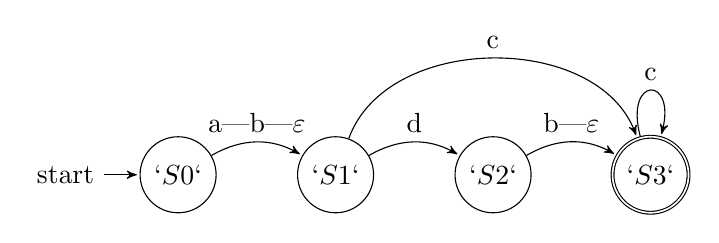
\begin{tikzpicture}[>=stealth',shorten >= 1pt,auto,node distance=2cm]
  \node[state,initial]        (S)                {`$S0$`};
  \node[state]                (q1) [right of=S]  {`$S1$`};
  \node[state]                (q2) [right of=q1] {`$S2$`};
  \node[state,accepting]      (q3) [right of=q2] {`$S3$`};

  \path[->] (S)  edge [bend left]  node {a|b|$\varepsilon$} (q1)
            (q1) edge [bend left=70]  node {c}              (q3)
                 edge [bend left]  node {d}                 (q2)
            (q2) edge [bend left]  node {b|$\varepsilon$}   (q3)
            (q3) edge [loop above] node {c}                 (q3);
\end{tikzpicture}

\item
Not quite sure if this is the expected answer, but if the program encounters a while loop without brackets as such:
\begin{lstlisting}
while(condition)
    singleOperation();
\end{lstlisting}
, the program will remove all code until a '\{' and a matching '\}' are encountered. As a result, the code snippet

\begin{lstlisting}
while(condition)
    singleOperation();
int a = 0;
int b = 1;
for(int i=0; i<10; ++i){
    oneOperation();
    anotherOperation();
}
++a;
++b;
\end{lstlisting}
will be trimmed down to

\begin{lstlisting}
++a;
++b;
\end{lstlisting}
.
\end{enumerate}

\section{Problem 2, Grammars}
\begin{enumerate}[a)]
\item
An ambiguous grammar is a grammar for which there exists a string that can have more than one leftmost derivation.\cite{wikiambi}

\item
The grammar is not ambiguous, as every string from the grammar can have only one leftmost derivation.

\item
A left recursive grammar is a grammar whose left-most symbol in any non-terminal production either immediately or through other non-terminal definitions rewrites to the same non-terminal production.\cite{wikilr}

\item
If i read the grammar correctly (Sp is a combination of the non-terminal S and a p), the grammar is left recursive.
\end{enumerate}
\begin{thebibliography}{9}

\bibitem{wikiambi}
  \url{http://en.wikipedia.org/wiki/Ambiguous_grammar}

\bibitem{wikilr}
  \url{http://en.wikipedia.org/wiki/Left_recursion}

\end{thebibliography}
\end{document}